\documentclass[11pt]{article}

\usepackage{times}
\usepackage{epsf}
\usepackage{epsfig}
\usepackage{amsmath, alltt, amssymb, xspace}
\usepackage{wrapfig}
\usepackage{fancyhdr}
\usepackage{url}
\usepackage{verbatim}
\usepackage{fancyvrb}

\usepackage{subfigure}
\usepackage{cite}
%\usepackage{cases}
%\usepackage{ltexpprt}
%\usepackage{verbatim}

%\topmargin      -0.70in  % distance to headers
%\headheight     0.2in   % height of header box
%\headsep        0.4in   % distance to top line
%\footskip       0.3in   % distance from bottom line

% Horizontal alignment
\topmargin      -0.50in  % distance to headers
\oddsidemargin  0.0in
\evensidemargin 0.0in
\textwidth      6.5in
\textheight     8.9in 


%\centerfigcaptionstrue

%\def\baselinestretch{0.95}


\newcommand\discuss[1]{\{\textbf{Discuss:} \textit{#1}\}}
%\newcommand\todo[1]{\vspace{0.1in}\{\textbf{Todo:} \textit{#1}\}\vspace{0.1in}}
\newtheorem{problem}{Problem}[section]
%\newtheorem{theorem}{Theorem}
%\newtheorem{fact}{Fact}
\newtheorem{define}{Definition}[section]
%\newtheorem{analysis}{Analysis}
\newcommand\vspacenoindent{\vspace{0.1in} \noindent}

%\newenvironment{proof}{\noindent {\bf Proof}.}{\hspace*{\fill}~\mbox{\rule[0pt]{1.3ex}{1.3ex}}}
%\newcommand\todo[1]{\vspace{0.1in}\{\textbf{Todo:} \textit{#1}\}\vspace{0.1in}}

%\newcommand\reducespace{\vspace{-0.1in}}
% reduce the space between lines
%\def\baselinestretch{0.95}

\newcommand{\fixmefn}[1]{ \footnote{\sf\ \ \fbox{FIXME} #1} }
\newcommand{\todo}[1]{
\vspace{0.1in}
\fbox{\parbox{6in}{TODO: #1}}
\vspace{0.1in}
}

\newcommand{\mybox}[1]{
\vspace{0.2in}
\noindent
\fbox{\parbox{6.5in}{#1}}
\vspace{0.1in}
}


\newcounter{question}
\setcounter{question}{1}

\newcommand{\myquestion} {{\vspace{0.1in} \noindent \bf Question \arabic{question}:} \addtocounter{question}{1} \,}

\newcommand{\myproblem} {{\noindent \bf Problem \arabic{question}:} \addtocounter{question}{1} \,}


\newcommand{\copyrightnoticeA}[1]{
\vspace{0.1in}
\fbox{\parbox{6in}{\small Copyright \copyright\ 2006 - 2014\ \ Wenliang Du, Syracuse University.\\ 
      The development of this document is partially funded by 
      the National Science Foundation's Course, Curriculum, and Laboratory 
      Improvement (CCLI) program under Award No. 0618680 and 0231122. 
      Permission is granted to copy, distribute and/or modify this document
      under the terms of the GNU Free Documentation License, Version 1.2
      or any later version published by the Free Software Foundation.
      A copy of the license can be found at http://www.gnu.org/licenses/fdl.html.}}
\vspace{0.1in}
}


\newcommand{\copyrightnotice}[1]{
\vspace{0.1in}
\fbox{\parbox{6in}{\small Copyright \copyright\ 2006 - 2014\ \ Wenliang Du, Syracuse University.\\
      The development of this document is/was funded by three grants from
      the US National Science Foundation: Awards No. 0231122 and 0618680 from
      TUES/CCLI and  Award No. 1017771 from Trustworthy Computing.
      This lab was imported into the Labtainer framework by the Naval Postgraduate 
      School, Center for Cybersecurity and Cyber Operations under National Science 
      Foundation Award No. 1438893.
      Permission is granted to copy, distribute and/or modify this document
      under the terms of the GNU Free Documentation License, Version 1.2
      or any later version published by the Free Software Foundation.
      A copy of the license can be found at http://www.gnu.org/licenses/fdl.html.}}
\vspace{0.1in}
}

\newcommand{\copyrightnoticeB}[1]{
\vspace{0.1in}
\fbox{\parbox{6in}{\small Copyright \copyright\ 2006 - 2014\ \ Wenliang Du, Syracuse University.\\
      The development of this document is/was funded by the following grants from
      the US National Science Foundation: No. 0231122, 0618680, and 1303306.
      Permission is granted to copy, distribute and/or modify this document
      under the terms of the GNU Free Documentation License, Version 1.2
      or any later version published by the Free Software Foundation.
      A copy of the license can be found at http://www.gnu.org/licenses/fdl.html.}}
\vspace{0.1in}
}


\newcommand{\nocopyrightnotice}[1]{
\vspace{0.1in}
\fbox{\parbox{6in}{\small  
      The development of this document is funded by 
      the National Science Foundation's Course, Curriculum, and Laboratory 
      Improvement (CCLI) program under Award No. 0618680 and 0231122. 
      Permission is granted to copy, distribute and/or modify this document.
      }}
\vspace{0.1in}
}

\newcommand{\idea}[1]{
\vspace{0.1in}
{\sf IDEA:\ \ \fbox{\parbox{5in}{#1}}}
\vspace{0.1in}
}

\newcommand{\questionblock}[1]{
\vspace{0.1in}
\fbox{\parbox{6in}{#1}}
\vspace{0.1in}
}


\newcommand{\minix}{{\tt Minix}\xspace}
\newcommand{\unix}{{\tt Unix}\xspace}
\newcommand{\linux}{{\tt Linux}\xspace}
\newcommand{\ubuntu}{{\tt Ubuntu}\xspace}
\newcommand{\selinux}{{\tt SELinux}\xspace}
\newcommand{\freebsd}{{\tt FreeBSD}\xspace}
\newcommand{\solaris}{{\tt Solaris}\xspace}
\newcommand{\windowsnt}{{\tt Windows NT}\xspace}
\newcommand{\setuid}{{\tt Set-UID}\xspace}
%\newcommand{\smx}{{\tt Smx}\xspace}
\newcommand{\smx}{{\tt Minix}\xspace}
\newcommand{\relay}{{\tt relay}\xspace}
\newcommand{\isys}{{\tt iSYS}\xspace}
\newcommand{\ilan}{{\tt iLAN}\xspace}
\newcommand{\iSYS}{{\tt iSYS}\xspace}
\newcommand{\iLAN}{{\tt iLAN}\xspace}
\newcommand{\iLANs}{{\tt iLAN}s\xspace}
\newcommand{\bochs}{{\tt Bochs}\xspace}

\newcommand\FF{{\mathcal{F}}}

\newcommand{\argmax}[1]{
\begin{minipage}[t]{1.25cm}\parskip-1ex\begin{center}
argmax
#1
\end{center}\end{minipage}
\;
}

\newcommand{\bm}{\boldmath}
\newcommand  {\bx}    {\mbox{\boldmath $x$}}
\newcommand  {\by}    {\mbox{\boldmath $y$}}
\newcommand  {\br}    {\mbox{\boldmath $r$}}


%\pagestyle{fancyplain}
%\lhead[\thepage]{\thesection}      % Note the different brackets!
%\rhead[\thesection]{SEED Laboratories}
%\lfoot[\fancyplain{}{}]{Syracuse University} 
%\cfoot[\fancyplain{}{}]{\thepage} 

\newcommand{\tstamp}{\today}   
%\lhead[\fancyplain{}{\thepage}]         {\fancyplain{}{\rightmark}}
%\chead[\fancyplain{}{}]                 {\fancyplain{}{}}
%\rhead[\fancyplain{}{\rightmark}]       {\fancyplain{}{\thepage}}
%\lfoot[\fancyplain{}{}]                 {\fancyplain{\tstamp}{\tstamp}}
%\cfoot[\fancyplain{\thepage}{}]         {\fancyplain{\thepage}{}}
%\rfoot[\fancyplain{\tstamp} {\tstamp}]  {\fancyplain{}{}}

\pagestyle{fancy}
%\lhead{\bfseries Computer Security Course Project}
\lhead{\bfseries SEED Labs}
\chead{}
\rhead{\small \thepage}
\lfoot{}
\cfoot{}
\rfoot{}

\usepackage{listings}
\usepackage{color}

\definecolor{dkgreen}{rgb}{0,0.6,0}
\definecolor{gray}{rgb}{0.5,0.5,0.5}
\definecolor{mauve}{rgb}{0.58,0,0.82}

\lstset{frame=tb,
  language=C,
  aboveskip=3mm,
  belowskip=3mm,
  showstringspaces=false,
  columns=flexible,
  basicstyle={\small\ttfamily},
  numbers=none,
  numberstyle=\tiny\color{gray},
  keywordstyle=\color{blue},
  commentstyle=\color{dkgreen},
  stringstyle=\color{mauve},
  breaklines=true,
  breakatwhitespace=true,
  tabsize=3
}



\begin{document}

\begin{center}
{\LARGE DNS Basics}
\vspace{0.1in}\\
\end{center}

\section{Overview}
This exercise introduces some basic functions and protocol elements of the Internet's
Domain Name Service (DNS).  The student will interact with an example enterprise having a local 
DNS server and several computers.

This exercise, (and manual), is not intended to replace instruction
or independent reading on DNS.

Broadly, a DNS provides a mapping between IP addresses and computer names.  DNS allows us to use
names such as ``google.com'' instead of remembering the IP address for google.  Computers generate
\textit{queries} such as ``What is the IP address for google.com?'' and send them to the DNS.  The DNS
generates a \textit{response} to the query, providing the requested information.  If the DNS does not itself
manage the requested information, the DNS forwards the query to another DNS for resolution.

This exercise is intended to provide
students with an environment with which they can observe 
traffic generated by DNS queries and responses.

This lab and its prerequisite knowlege provide background for other Labtainer networking exercises 
including a lab on local DNS poisoning attacks.

This lab exercises includes use of the Linux command line (shell), and Wireshark.

\section{Lab Environment}
This lab runs in the Labtainer framework,
available at http://nps.edu/web/c3o/labtainers.
That site includes links to a pre-built virtual machine
that has Labtainers installed, however Labtainers can
be run on any Linux host that supports Docker containers.

From your labtainer-student directory start the lab using:
\begin{verbatim}
    labtainer dns
\end{verbatim}
\noindent A link to this lab manual will be displayed.  

\section{Network Configuration}
The lab includes networked components as illustrated in figure \ref{fig:topology}.  Note that all of
the IP addresses are local.  
The DNS is configured to provide authoritative naming for devices within the domain called
\textit{example.com}.  
In this topology, the DNS is only providing local naming and forwards any
non-local requests to the gateway.


\begin{figure}[H]
\begin{center}
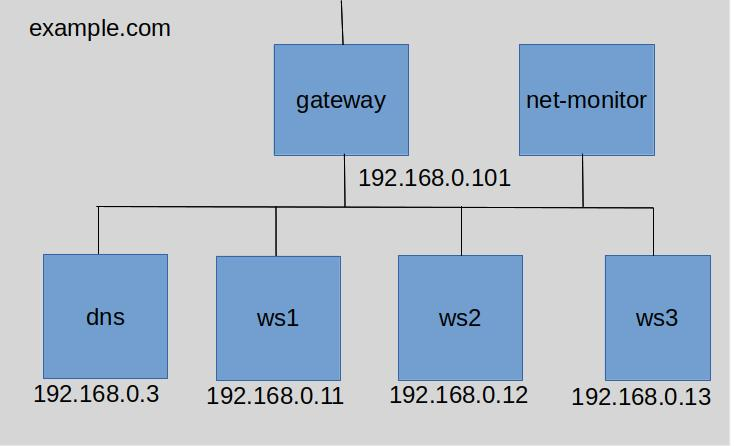
\includegraphics [width=0.8\textwidth]{dns.jpg}
\end{center}
\caption{Network topology for the DNS lab}
\label{fig:topology}
\end{figure}


\section{Lab Tasks}
\subsection{Explore}
The DNS is configured to provide naming devices within {\tt example.com}.  Initially, it is configured
to name {\tt ws1} and {\tt ws2}.  And the {\tt ws1} and {\tt ws2} computers
are configured to use the DNS as their name server.  The {\tt ws3} computer is not yet configured.  Use the 
{\tt ping} command see how you can use the names {\tt ws1} and {\tt ws2} in place of IP addresses.  For
example, on {\tt ws1} type:
\begin{verbatim}
    ping ws2 -c 2
\end{verbatim} 
\noindent Note that if you try to ping {\tt ws3}, if fails.  However you can ping {\tt ws3} using its 
IP address.

You will update the DNS and {\tt ws3} later in this exercise.  But first, we will review some of the DNS protocol.

\subsection{View DNS traffic}
The lab environment includes a {\tt new-monitor} computer that captures all traffic on the local network.
It collects all network traffic into a file within its {\tt /taps} directory.  Go to the terminal for the
{\tt net-monitor} computer and list the content of that directory to see that it is a PCAP file:
\begin{verbatim}
   ls -l /taps
\end{verbatim}
\noindent You can start Wireshark and view that PCAP file as it is updated by using this command on the
{\tt network-monitor} component:
\begin{verbatim}
   sharktap lan.pcap
\end{verbatim}
After Wireshark comes up, scroll backward and find the intitial DNS traffic.  Note that this conversation
occurs between the local DNS and some external DNS, and is used by the local DNS for initialization.  Scroll forward to the next DNS protocol conversation, which should be between the {\tt ws1} component and the DNS.

Select the first packet of that exchange, i.e., the one from your {\tt ws1} component and then view the
details of the protocol as presented by Wireshark in the middle pane.  Find the ``queries'' block and
view the query.   Note how the query is asking for the IP address of \textit{ws2.example.com}, yet you only
provided the name {\tt ws2} to the ping command.  So, where did the {\tt example.com} name come from?  Within
this Linux system, that information is provided as the \textit{search} directive within the 
{\tt /etc/resolv.conf} file on the computer that is issuing the DNS query.  Go to {\tt ws1} and view that file:
\begin{verbatim}
    cat /etc/resolv.conf
\end{verbatim}
\noindent That search directive tells the computer to tack the name {\tt example.com} onto names that do
not end with a domain suffix such as \textit{.com}, e.g., are just names like {\tt ws2}.  Note the {\tt resolv.conf} file
also contains a \textit{nameserver} directive.  This tells the computer the IP address of its DNS service.

Note how there is a 2nd query from {\tt ws1} to the DNS.  That is to retrieve and IPV6 address.  Ignore that 
for this lab.  The next packet should be a response from the DNS to ws1.  View its protocol elements.
Note how it repeats the query, but also has an \textit{answers} section.  View that to see the response from
the DNS.  The next packet is the DNS response to the IPV6 query, which can be ignored for this lab.

\subsection{Missing names}
The {\tt ws3} computer is not yet defined in the DNS.  Test this by trying to ping {\tt ws3} from {\tt ws1}:
\begin{verbatim}
    ping ws3 -c 2
\end{verbatim}
Find the reply from the DNS and note the respone flags indicates there is ``no such name''.
Note that {\tt ws1} then tries another query, this time asking for {\tt ws3} instead of {\tt ws3.example.com}.
Since this query is not for a name within the {\tt example.com} domain, the local DNS farms out the request
to another DNS via the gateway (192.168.0.101).  That DNS responds with ``No such name''.

\subsection{Missing DNS}
Go to {\tt ws3} and try to ping {\tt ws1}:
\begin{verbatim}
    ping ws1 -c 2
\end{verbatim}
\noindent Note the lack of traffic in Wireshark.  The {\tt ws3} computer has no defined DNS, so it does not
know where to send a DNS query.  Use {\tt vi} or {\tt nano} to edit the {\tt /etc/resolv.conf} file so that
it matches those in {\tt ws1} and {\tt ws2}.

Then try pinging {\tt ws1} again.  Now that {\tt ws3} has the address of its {\tt nameserver}, it can use
names instead of IP addresses.

\subsection{Add missing name}
In this section, you will update the DNS so that it can provide the IP address of {\tt ws3}.
The DNS is provided by the \textit{bind9} service on the dns computer.  Information about this service and
its configuration files can be found at \url{https://ubuntu.com/server/docs/service-domain-name-service-dns}.
This section refers to the primary files used to configure the DNS.  

The starting point is the {\tt /etc/named.conf} file\footnote{The word \textit{named} derives from
the fact that this service is sometimes referred to as the \textit{name daemon}}.  View that file and note that it simply includes
three other files.  The second file, {\tt named.conf.local} is where the local names are defined.
View that file.  As you see, this DNS manages names defined in a single local file, {\tt example.conf}. 
View that file.  At last, a file that does not just include other files!  This file includes to \textit{zone}
sections.  The first defines how the DNS will respond to queries of names within the {\tt example.com}
domain, or {\tt zone}.  The second entry defines a \textit{reverse name lookup}, which is another function of
the DNS via which a computer can query the name associated with an IP address, e.g., ``What is the name of
the device having IP address 192.168.0.1?''.

View the file named in the first section, i.e., {\tt /var/named/example.com.zone}.  The first set of lines
in that file reflect various configuration options for handing queries for the {\tt example.com} domain,
including things like timeout values.  Toward the bottom of the file you will see entries that look like
a mapping of computer names to IP addresses.  There are entries for {\tt ws1} and {\tt ws2}, but not one
for {\tt ws3}.  Add one for {\tt ws3}.

Then direct your attention to the second section of the {\tt example.conf} file, i.e., the reverse name
looking information.
Note the funny looking zone name: \textit{0.168.192.in-addr.arpa}, and how the first part of the name
includes the {\tt example.com} domain address, but in reverse.  This indicates that if the first three
octets of an IP address match those three octets, then the remaining octet will name the computer.
View the named file, i.e., {\tt /var/named/192.168.0.0}. Observe how the last two entries identify the 
last octet in the IP addresses of {\tt ws2} and {\tt ws3}.  Add an entry for {\tt ws3}.

\subsection{Apply and test DNS changes}
After modifying the DNS configuration files, the DNS service must be restarted:
\begin{verbatim}
   sudo systemctl restart bind9
\end{verbatim}

\noindent Then try to ping {\tt ws3} from {\tt ws1}.  You should be able to see the resulting DNS query
and response in Wireshark.

\section{Quiz}
Go to the terminal on your Linux system that was used to start the lab and type:
\begin{verbatim}
    quiz -l dns -q post
\end{verbatim}
\noindent and answer the quiz questions to test your knowledge of what you have done in this lab.

\section{Submission}
After finishing the lab, go to the terminal on your Linux system that was used to start the lab and type:
\begin{verbatim}
    stoplab 
\end{verbatim}
When you stop the lab, the system will display a path to the zipped lab results on your Linux system.  Provide that file to 
your instructor, e.g., via the Sakai site.


\copyrightnotice

\end{document}
